%!TEX root = ./main.tex

\section{Architecture Across Generations}

% SECTION TIMING: 20:00--52:00. Follow one call/packet; abbreviations are roles, not a memorization list.

\begin{frame}{1G connected radio voice to the telephone network}
  \begin{columns}[T,onlytextwidth]
    \column{0.56\textwidth}
      \centering
      \begin{tikzpicture}[node distance=0.55cm,scale=0.76,transform shape]
        \node[netnode,minimum width=1.55cm] (phone) {Mobile\\phone};
        \node[netnode,minimum width=1.65cm,right=of phone] (bs) {Base\\station};
        \node[corenode,minimum width=1.75cm,right=of bs] (mtso) {MTSO};
        \node[corenode,minimum width=1.65cm,right=of mtso] (pstn) {PSTN};
        \draw[flow] (phone)--(bs);
        \draw[flow] (bs)--(mtso);
        \draw[flow] (mtso)--(pstn);
        \node[align=center,font=\scriptsize,text width=5.2cm] at (2.8,-1.35)
          {A circuit stays reserved while the call is active.};
      \end{tikzpicture}
      \vspace{0.4em}
      {\scriptsize
        MTSO = Mobile Telephone Switching Office\\
        PSTN = Public Switched Telephone Network\par}
    \column{0.40\textwidth}
      \large\textbf{The path was a circuit.}

      \vspace{0.4em}
      \small
      \begin{itemize}\itemsep4pt
        \item Analog radio in the cell
        \item MTSO linked the towers
        \item PSTN carried the call
      \end{itemize}
  \end{columns}

  \vspace{0.5em}
  \takeaway{A mobile call was still a telephone call.}
\end{frame}

% Prediction (60 s): ask who notices the weakening signal and who reroutes the call.
\begin{frame}{Mobility means changing the network while using it}
  \begin{columns}[T,onlytextwidth]
    \column{0.52\textwidth}
      \centering
      \begin{tikzpicture}[scale=0.82,transform shape]
        \draw[draw=ranblue!55,fill=blue!3] (0,0) circle (1.35);
        \draw[draw=ranblue!55,fill=blue!3] (2.6,0) circle (1.35);
        \node[netnode,minimum width=1.2cm] at (0,0) {Cell A};
        \node[netnode,minimum width=1.2cm] at (2.6,0) {Cell B};
        \node[corenode,minimum width=1.75cm] (core) at (1.3,-1.95) {Switch /\\controller};
        \draw[flow] (0,-0.45)--(core);
        \draw[flow] (2.6,-0.45)--(core);
        \draw[flow,draw=ranpurple] (-0.9,1.85)--(3.5,1.85);
        \node[font=\scriptsize,anchor=north] at (-0.15,1.75) {moving call};
        \filldraw[fill=coreorange,draw=coreorange] (1.3,1.85) circle (2.5pt);
        \node[font=\scriptsize,align=center,anchor=south] at (1.5,2.0) {handoff decision};
      \end{tikzpicture}
    \column{0.44\textwidth}
      \large\textbf{A moving car raises\\three questions:}

      \vspace{0.4em}
      \small
      \begin{itemize}\itemsep4pt
        \item Who measures the signal?
        \item Who picks the next cell?
        \item Who keeps the call alive?
      \end{itemize}
  \end{columns}

  \qa{What goes wrong if the handoff is late? If it is too early?}
     {Late, the call drops while the old cell fades. Too early, the phone
      ping-pongs between cells and spends signaling on a move it did not need.}
\end{frame}

\begin{frame}{2G split the base station into radio and control}
  \vspace{0.4em}
  \centering
  \begin{tikzpicture}[node distance=0.45cm,scale=0.82,transform shape]
    \node[netnode] (ms) {Mobile\\station};
    \node[netnode,right=of ms] (bts) {BTS};
    \node[netnode,right=of bts] (bsc) {BSC};
    \node[corenode,right=of bsc] (msc) {MSC};
    \node[corenode,above=0.6cm of msc] (db) {HLR / VLR\\AuC};
    \node[corenode,right=of msc] (pstn) {PSTN};
    \draw[flow] (ms)--(bts);
    \draw[flow] (bts)--(bsc);
    \draw[flow] (bsc)--(msc);
    \draw[flow] (msc)--(pstn);
    \draw[flow,dashed] (msc)--(db);
  \end{tikzpicture}

  \vspace{0.9em}
  {\small
  \begin{tabular}{@{}r@{\hspace{0.6em}}l@{}}
    \textbf{BTS} & Base Transceiver Station\\
    \textbf{BSC} & Base Station Controller\\
    \textbf{MSC} & Mobile Switching Center\\
    \textbf{HLR / VLR} & Home / Visitor Location Register\\
    \textbf{AuC} & Authentication Center\\
  \end{tabular}\par}

  \vspace{0.7em}
  \takeaway{Digital identities made roaming scalable.}
\end{frame}

\begin{frame}{The SIM became a network passport}
  \begin{columns}[T,onlytextwidth]
    \column{0.38\textwidth}
      \centering
      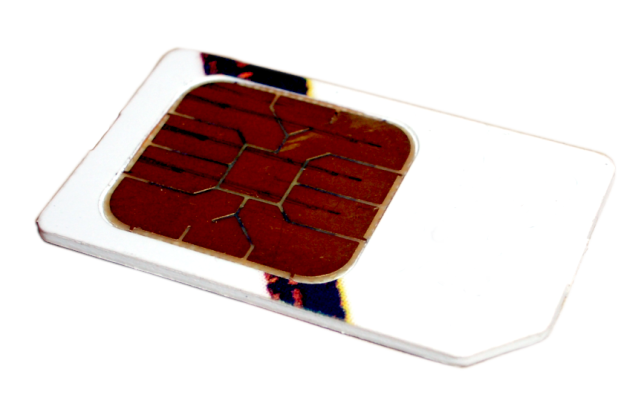
\includegraphics[width=0.92\linewidth]{figure/xg/sim_card.png}
      \source{https://commons.wikimedia.org/wiki/File:Sim_card.png}{GSM SIM card}
    \column{0.58\textwidth}
      \large\textbf{Home network}

      \normalsize knows your subscription,\\number, and credentials.

      \vspace{0.8em}
      \large\textbf{Visited network}

      \normalsize knows where to reach you\\right now.
  \end{columns}

  \qa{If you replace the phone but keep the SIM, what changed in the network?}
     {Almost nothing. The network still authenticates the same subscriber record,
      so your number, your subscription, and your roaming state survive. Only the
      device identity and its radio capabilities changed.}
\end{frame}

\begin{frame}{A call can find you even when you leave home}
  \begin{columns}[T,onlytextwidth]
    \column{0.56\textwidth}
      \centering
      \begin{tikzpicture}[node distance=0.55cm,scale=0.70,transform shape]
        \node[corenode,minimum width=2.25cm] (home) {Home network\\HLR};
        \node[corenode,minimum width=2.25cm,right=2.6cm of home] (visit) {Visited network\\VLR / MSC};
        \node[netnode,below=0.75cm of visit] (bob) {Bob's phone};
        \node[netnode,below=0.75cm of home] (mary) {Mary};
        \draw[flow] (bob)--node[right,font=\scriptsize]{register}(visit);
        \draw[flow,dashed] (visit)--node[above,font=\scriptsize]{update location}(home);
        \draw[flow] (mary)--node[left,font=\scriptsize]{call Bob}(home);
        \draw[flow] (home)--node[below,font=\scriptsize]{route call}(visit);
      \end{tikzpicture}
    \column{0.40\textwidth}
      \large\textbf{Bob visits\\another city.}

      \vspace{0.4em}
      \small
      \begin{enumerate}\itemsep5pt
        \item Bob registers there.
        \item The HLR is updated.
        \item Mary's call is routed.
      \end{enumerate}
  \end{columns}

  \vspace{0.5em}
  \takeaway{Mobility also needs a database.}
\end{frame}

\begin{frame}{GPRS was an Internet sidecar}
  \vspace{-0.3em}
  {\small GPRS = General Packet Radio Service, packet data added onto GSM.\par}
  \vspace{0.3em}
  \centering
  \begin{tikzpicture}[node distance=0.45cm,scale=0.78,transform shape]
    \node[netnode] (phone) {Phone};
    \node[netnode,right=of phone] (bss) {BSS\\BTS+BSC};
    \node[corenode,right=of bss,yshift=0.85cm] (msc) {MSC\\voice};
    \node[corenode,right=of bss,yshift=-0.85cm] (sgsn) {SGSN};
    \node[corenode,right=of sgsn] (ggsn) {GGSN};
    \node[netnode,right=of ggsn] (inet) {Internet};
    \node[netnode,right=of msc] (pstn) {PSTN};
    \draw[flow] (phone)--(bss);
    \draw[flow] (bss)--(msc);
    \draw[flow] (msc)--(pstn);
    \draw[flow,draw=ranblue] (bss)--(sgsn);
    \draw[flow,draw=ranblue] (sgsn)--(ggsn);
    \draw[flow,draw=ranblue] (ggsn)--(inet);
  \end{tikzpicture}

  \glossline{SGSN = Serving GPRS Support Node \quad
    GGSN = Gateway GPRS Support Node}

  \vspace{0.6em}
  \raggedright
  \begin{itemize}\itemsep4pt
    \item Voice still used the MSC path.
    \item Packet data used SGSN and GGSN.
    \item The phone gained a standing route to the Internet.
  \end{itemize}

  \vspace{0.3em}
  \takeaway{Packet data arrived next to voice, not instead of it.}
\end{frame}

\begin{frame}{3G changed the radio faster than the architecture}
  \centering
  \begin{tikzpicture}[node distance=0.45cm]
    \node[netnode] (ue) {UE};
    \node[netnode,right=of ue] (nb) {NodeB};
    \node[netnode,right=of nb] (rnc) {RNC};
    \node[corenode,right=of rnc,yshift=0.95cm] (msc) {MSC\\voice};
    \node[corenode,right=of rnc,yshift=-0.95cm] (sgsn) {SGSN/GGSN\\data};
    \draw[flow] (ue) -- (nb);
    \draw[flow] (nb) -- (rnc);
    \draw[flow] (rnc) -- (msc);
    \draw[flow] (rnc) -- (sgsn);
  \end{tikzpicture}

  \vspace{0.5em}
  {\scriptsize NodeB = 3G radio node \quad\textbullet\quad RNC = Radio Network Controller\par}

  \vspace{0.8em}
  \raggedright
  \begin{itemize}\itemsep4pt
    \item UMTS/WCDMA raised mobile-data capability.
    \item NodeB and RNC echoed the BTS/BSC split.
    \item Circuit voice and packet data lived side by side.
  \end{itemize}
  \source{https://www.3gpp.org/technologies/3g}{3GPP 3G overview}
\end{frame}

\begin{frame}{3G carried two networks in one trench coat}
  \vspace{0.5em}
  \begin{columns}[T,onlytextwidth]
    \column{0.48\textwidth}
      \centering
      \Huge\textcolor{coreorange}{\textbf{Voice}}

      \vspace{0.6em}
      \Large Circuit switched

      \vspace{0.5em}
      \normalsize MSC and the telephone world
    \column{0.48\textwidth}
      \centering
      \Huge\textcolor{ranblue}{\textbf{Data}}

      \vspace{0.6em}
      \Large Packet switched

      \vspace{0.5em}
      \normalsize SGSN/GGSN and the Internet
  \end{columns}

  \vspace{1.2em}
  \takeaway{Running both worlds at once worked. It was not simple.}
\end{frame}

% Classroom check (90 s): students match names before the answers appear orally.
\begin{frame}{Can you match the tower name to the generation?}
  \vspace{0.5em}
  \begin{columns}[T,onlytextwidth]
    \column{0.46\textwidth}
      \large
      \begin{enumerate}\itemsep4pt
        \item BTS
        \item NodeB
        \item eNodeB
        \item gNodeB
      \end{enumerate}
    \column{0.50\textwidth}
      \large
      \begin{itemize}\itemsep4pt
        \item 2G GSM
        \item 3G UMTS
        \item 4G LTE
        \item 5G NR
      \end{itemize}
  \end{columns}

  \glossline{GSM = Global System for Mobile Communications \quad NR = New Radio\\
    The prefixes are generational: e = evolved (LTE), g = next generation (5G).}

  \vspace{0.9em}
  \qa{Which generation removed the separate radio controller?}
     {4G. The eNodeB absorbed the scheduling and handover control that the RNC
      used to own, so LTE has no separate controller box in the main path.}
\end{frame}

\begin{frame}{4G flattened the RAN}
  \centering
  \begin{tikzpicture}[node distance=0.5cm,scale=0.8,transform shape]
    \node[netnode] (ue) {UE};
    \node[netnode,right=of ue] (enb1) {eNodeB};
    \node[netnode,below=0.6cm of enb1] (enb2) {eNodeB};
    \node[corenode,right=1.0cm of enb1] (epc) {EPC};
    \node[netnode,right=of epc] (net) {Internet};
    \draw[flow] (ue)--(enb1);
    \draw[flow] (enb1)--(epc);
    \draw[flow] (enb2)--(epc);
    \draw[flow,dashed] (enb1)--node[right,font=\scriptsize]{X2}(enb2);
    \draw[flow] (epc)--(net);
  \end{tikzpicture}

  \glossline{No separate RNC sits in the main LTE path. \quad
    EPC = Evolved Packet Core}

  \vspace{0.6em}
  \raggedright
  \begin{itemize}\itemsep4pt
    \item The eNodeB absorbed the radio control that lived in the RNC.
    \item Neighboring eNodeBs coordinate directly over X2.
    \item The core became the Evolved Packet Core.
  \end{itemize}

  \vspace{0.3em}
  \takeaway{Fewer boxes in the path.\\More logic inside the base station.}
\end{frame}

\begin{frame}{The EPC turned the core into packet plumbing}
  \vspace{0.2em}
  \centering
      \begin{tikzpicture}[node distance=0.48cm,scale=0.78,transform shape]
        \node[netnode] (ue) {UE};
        \node[netnode,right=of ue] (enb) {eNodeB};
        \node[corenode,right=of enb,yshift=0.75cm] (mme) {MME};
        \node[corenode,right=of mme] (hss) {HSS};
        \node[corenode,right=of enb,yshift=-0.75cm] (sgw) {SGW};
        \node[corenode,right=of sgw] (pgw) {PGW};
        \node[netnode,right=of pgw] (inet) {Internet};
        \draw[flow] (ue)--(enb);
        \draw[flow,dashed] (enb)--(mme);
        \draw[flow,dashed] (mme)--(hss);
        \draw[flow,draw=ranblue] (enb)--(sgw);
        \draw[flow,draw=ranblue] (sgw)--(pgw);
        \draw[flow,draw=ranblue] (pgw)--(inet);
      \end{tikzpicture}

  \glossline{dashed = control signaling \quad\textbullet\quad solid blue = user data}

  \vspace{0.7em}
  {\small
  \begin{tabular}{@{}r@{\hspace{0.6em}}l@{}}
    \textbf{MME} & Mobility Management Entity\\
    \textbf{HSS} & Home Subscriber Server\\
    \textbf{SGW} & Serving Gateway\\
    \textbf{PGW} & Packet Data Network Gateway\\
  \end{tabular}\par}

  \vspace{0.7em}
  \takeaway{Learn the jobs, not the acronym list.}
\end{frame}

\begin{frame}{Control asks; the user plane moves packets}
  \centering
  \begin{tikzpicture}[node distance=0.75cm]
    \node[netnode] (ue) {UE};
    \node[netnode,right=of ue] (enb) {eNodeB};
    \node[corenode,right=of enb,yshift=0.85cm] (mme) {MME\\control};
    \node[corenode,right=of enb,yshift=-0.85cm] (gw) {S/PGW\\user data};
    \node[netnode,right=of gw] (net) {Internet};
    \draw[flow,dashed] (ue) -- (enb);
    \draw[flow,dashed] (enb) -- (mme);
    \draw[flow,draw=ranblue] (ue) to[bend right=18] (enb);
    \draw[flow,draw=ranblue] (enb) -- (gw);
    \draw[flow,draw=ranblue] (gw) -- (net);
  \end{tikzpicture}

  \vspace{1.2em}
  \begin{columns}[T,onlytextwidth]
    \column{0.47\textwidth}
      \Large\textbf{Control plane}

      \normalsize attach, authenticate,\\move, establish a bearer
    \column{0.49\textwidth}
      \Large\textbf{User plane}

      \normalsize carry the voice, video,\\game, or web packets
  \end{columns}

  \vspace{0.8em}
  \takeaway{Separating the two planes\\lets each one scale on its own.}
\end{frame}

% Discussion (60 s): why did an early LTE phone sometimes fall back to 3G for a call?
\begin{frame}{In 4G, a phone call had to become an Internet app}
  \vspace{0.4em}
  \begin{columns}[T,onlytextwidth]
    \column{0.46\textwidth}
      \centering
      \Huge\textcolor{gray}{\textbf{Early LTE}}

      \vspace{0.8em}
      \large Data on LTE\par
      \vspace{0.3em}
      Voice falls back to 2G/3G
    \column{0.50\textwidth}
      \centering
      \Huge\textcolor{ranblue}{\textbf{VoLTE}}

      \vspace{0.8em}
      \large Voice as a managed IP service\par
      \vspace{0.3em}
      IMS provides call control
  \end{columns}

  \glossline{VoLTE = Voice over LTE \quad IMS = IP Multimedia Subsystem,
    the part of the core that sets up and controls calls}

  \vspace{1.0em}
  \qa{Why was ``all-IP'' a bigger change than making the radio faster?}
     {Speed is one number. All-IP changed the structure: one packet transport
      carries everything, and voice becomes an application on top of it instead
      of its own circuit-switched network.}
\end{frame}

\begin{frame}{5G made the core look more like a cloud platform}
  \begin{columns}[T,onlytextwidth]
    \column{0.56\textwidth}
      \centering
      \begin{tikzpicture}
        \node[corenode,minimum width=1.25cm,font=\scriptsize\bfseries] (amf) at (0,1.25) {AMF};
        \node[corenode,minimum width=1.25cm,font=\scriptsize\bfseries] (smf) at (1.8,1.25) {SMF};
        \node[corenode,minimum width=1.25cm,font=\scriptsize\bfseries] (ausf) at (3.6,1.25) {AUSF};
        \node[corenode,minimum width=1.25cm,font=\scriptsize\bfseries] (udm) at (0,0.15) {UDM};
        \node[corenode,minimum width=1.25cm,font=\scriptsize\bfseries] (pcf) at (1.8,0.15) {PCF};
        \node[corenode,minimum width=1.25cm,font=\scriptsize\bfseries] (nrf) at (3.6,0.15) {NRF};
        \node[oranode,minimum width=5.35cm,minimum height=0.58cm,font=\scriptsize\bfseries] (bus) at (1.8,-0.95) {Service-based interfaces};
        \foreach \n in {amf,smf,ausf,udm,pcf,nrf} \draw[thin,draw=coreorange] (\n) -- (bus);
        \node[netnode,minimum width=1.35cm,font=\scriptsize\bfseries] (ran) at (-0.05,-2.25) {RAN};
        \node[corenode,minimum width=1.35cm,font=\scriptsize\bfseries] (upf) at (1.8,-2.25) {UPF};
        \node[netnode,minimum width=1.55cm,font=\scriptsize\bfseries] (data) at (3.65,-2.25) {Data net};
        \draw[flow] (ran)--(upf); \draw[flow] (upf)--(data);
      \end{tikzpicture}

      \vspace{0.3em}
      {\scriptsize The SMF steers the UPF over the N4 interface.\par}
      \source{https://www.nokia.com/asset/i/210365/}{Nokia 5G Core Service Based Architecture}
    \column{0.40\textwidth}
      \small
      \plainterm{AMF}{Access + Mobility}\par\vspace{0.35em}
      \plainterm{SMF}{Session Management}\par\vspace{0.35em}
      \plainterm{UPF}{User Plane Function}\par\vspace{0.35em}
      \plainterm{AUSF/UDM}{identity}\par\vspace{0.35em}
      \plainterm{PCF}{policy}\par\vspace{0.35em}
      \plainterm{NRF}{service registry}
  \end{columns}

  \vspace{0.3em}
  \takeaway{Core functions now discover and call each other as services.}
\end{frame}

\begin{frame}{A 5G radio does not guarantee a 5G core}
  \vspace{-0.2em}
  {\small NSA = Non-Standalone \quad SA = Standalone \quad
    QoS = Quality of Service\par}
  \vspace{0.3em}
  \begin{columns}[T,onlytextwidth]
    \column{0.48\textwidth}
      \centering
      \Large\textbf{NSA}

      \vspace{0.6em}
      \begin{tikzpicture}[node distance=0.35cm,scale=0.86,transform shape]
        \node[netnode] (lte) {LTE anchor};
        \node[netnode,below=of lte] (nr) {5G NR};
        \node[corenode,right=of lte] (epc) {4G EPC};
        \draw[flow] (lte) -- (epc);
        \draw[flow] (nr) -- (lte);
      \end{tikzpicture}

      \vspace{0.6em}
      \small The phone shows 5G.\\Control still runs through\\LTE and the 4G core.
    \column{0.48\textwidth}
      \centering
      \Large\textbf{SA}

      \vspace{0.6em}
      \begin{tikzpicture}[node distance=0.35cm,scale=0.86,transform shape]
        \node[netnode] (nr) {5G NR};
        \node[corenode,right=of nr] (gc) {5G Core};
        \draw[flow] (nr) -- (gc);
      \end{tikzpicture}

      \vspace{1.35em}
      \small A 5G radio on a 5G core.\\Slicing, edge, and new QoS\\become possible.
  \end{columns}

  \vspace{0.6em}
  \takeaway{The icon reports the radio.\\The features come from the core.}
  \source{https://about.att.com/blogs/2025/5g-standalone-nationwide.html}{AT\&T: ``Not all 5G is created equal,'' 2025}
\end{frame}

\begin{frame}{The 5G base station can be split across locations}
  \vspace{0.3em}
  \centering
  \begin{tikzpicture}[node distance=1.15cm,scale=0.80,transform shape]
    \node[netnode,minimum width=1.30cm] (ue) {UE};
    \node[netnode,minimum width=1.70cm,right=of ue,font=\scriptsize\bfseries] (ru) {RU};
    \node[netnode,minimum width=1.70cm,right=of ru,font=\scriptsize\bfseries] (du) {DU};
    \node[netnode,minimum width=1.70cm,right=of du,font=\scriptsize\bfseries] (cu) {CU};
    \node[corenode,minimum width=1.70cm,right=of cu,font=\scriptsize\bfseries] (core) {5G Core};
    \draw[flow] (ue)--node[above,font=\tiny]{radio}(ru);
    \draw[flow] (ru)--node[above,font=\tiny]{fronthaul}(du);
    \draw[flow] (du)--node[above,font=\tiny]{F1}(cu);
    \draw[flow] (cu)--node[above,font=\tiny]{N2/N3}(core);
    \node[font=\scriptsize,below=0.35cm of ru,align=center] {RF +\\lower PHY};
    \node[font=\scriptsize,below=0.35cm of du,align=center] {upper PHY\\MAC / RLC};
    \node[font=\scriptsize,below=0.35cm of cu,align=center] {PDCP\\RRC / SDAP};
  \end{tikzpicture}

  \vspace{0.7em}
  {\small One gNodeB can be a system spread across a tower, a cabinet, and a data center.\par}

  \glossline{RU / DU / CU = Radio / Distributed / Central Unit\\
    PHY = physical layer \quad MAC = Medium Access Control \quad
    RLC = Radio Link Control\\
    PDCP = Packet Data Convergence Protocol \quad RRC = Radio Resource Control\\
    SDAP = Service Data Adaptation Protocol}

  \qa{Who owns each box, and who owns the interfaces between them?}
     {In a classic RAN, one vendor owns all of it. Splitting the base station only
      helps if the seams between the pieces are specified well enough for a second
      vendor to plug in.}
\end{frame}
